\documentclass{article}
\usepackage[T1]{fontenc}
\usepackage[utf8]{inputenc}
\usepackage[margin=2cm]{geometry}
\usepackage{graphicx}
\usepackage{parskip}
\usepackage{booktabs}
\usepackage{amsmath}

\title{Zadanie 4 - Raport}
\author{Jan Stusio}
\date{Maj 2024}

\begin{document}

\maketitle

\section{Wstęp}

Celem zadania jest zbadanie własności klasyfikatora SVM (z ang. Support Vector Machine, po pol. Maszyny wektorów nośnych) oraz drzewa decyzyjnego.
Model SVM ma przewidywać wartości dyskretne $-$ klasy, gdzie poszukujemy funkcji decyzyjnej, która najlepiej oddziela dane.
Gdy zadanie jest liniowo nieseparowalne, stosuje się funkcję jądra, która mapuje dane do przestrzeni o wyższej wymiarowości. 
Drzewo decyzyjne jest modelem, który w każdym węźle dokonuje podziału na podzbiory, aż do osiągnięcia warunku stopu.


Klasyfikator wskazuje dla danego x najbardziej prawdopodobną wartość y

\section{Implementacja}

Implementacja ładowania zbioru danych oraz treningu i ewaluacji przy wykorzystaniu walidacji krzyżowej (z założeniem 5 podziałów zbioru danych).

\section{Badania}

\subsection{Badania wpływu parametrów w klasyfikatorze SVM\@:}

\quad 1. Siła regularyzacji

\quad 2. Funkcja jądra

\quad 3. Liczba iteracji ( bardzo niski parametr tol w funkcji sklearn.svm.SVC)

\subsection{Badania wpływu parametrów w drzewie decyzyjnym\@:}

\quad 1. Kryterium oceny

\quad 2. Technika podziału węzła

\quad 3. Maksymalna głębokość drzewa

\pagebreak

\section{Wyniki eksperymentów}

\subsection{Tabela porównująca wyniki klasyfikatorów SVM i drzewa decyzyjnego.}

\begin{tabular}{llllr}
\toprule
Model & Parameter & Value & Metric & Score \\
\midrule
SVC & C & 0.100000 & accuracy & 0.940000 \\
SVC & C & 1.000000 & accuracy & 0.966667 \\
SVC & C & 10.000000 & accuracy & 0.966667 \\
SVC & C & 100.000000 & accuracy & 0.960000 \\
SVC & C & 0.100000 & \text{precision\_macro} & 0.941717 \\
SVC & C & 1.000000 & \text{precision\_macro} & 0.967222 \\
SVC & C & 10.000000 & \text{precision\_macro} & 0.971453 \\
SVC & C & 100.000000 & \text{precision\_macro} & 0.965527 \\
SVC & C & 0.100000 & \text{recall\_macro} & 0.943990 \\
SVC & C & 1.000000 & \text{recall\_macro} & 0.967222 \\
SVC & C & 10.000000 & \text{recall\_macro} & 0.964921 \\
SVC & C & 100.000000 & \text{recall\_macro} & 0.956402 \\
SVC & C & 0.100000 & F1 & 0.940851 \\
SVC & C & 1.000000 & F1 & 0.966981 \\
SVC & C & 10.000000 & F1 & 0.965934 \\
SVC & C & 100.000000 & F1 & 0.957527 \\
SVC & kernel & linear & accuracy & 0.966667 \\
SVC & kernel & poly & accuracy & 0.966667 \\
SVC & kernel & rbf & accuracy & 0.960000 \\
SVC & kernel & sigmoid & accuracy & 0.046667 \\
SVC & kernel & linear & \text{precision\_macro} & 0.971082 \\
SVC & kernel & poly & \text{precision\_macro} & 0.971082 \\
SVC & kernel & rbf & \text{precision\_macro} & 0.965527 \\
SVC & kernel & sigmoid & \text{precision\_macro} & 0.027103 \\
SVC & kernel & linear & \text{recall\_macro} & 0.963810 \\
SVC & kernel & poly & \text{recall\_macro} & 0.963810 \\
SVC & kernel & rbf & \text{recall\_macro} & 0.956402 \\
SVC & kernel & sigmoid & \text{recall\_macro} & 0.056270 \\
SVC & kernel & linear & F1 & 0.964347 \\
SVC & kernel & poly & F1 & 0.964347 \\
SVC & kernel & rbf & F1 & 0.957527 \\
SVC & kernel & sigmoid & F1 & 0.034511 \\
SVC & iteration & 100 & accuracy & 0.046667 \\
SVC & iteration & 1000 & accuracy & 0.046667 \\
SVC & iteration & 10000 & accuracy & 0.046667 \\
SVC & iteration & 100 & \text{precision\_macro} & 0.027103 \\
SVC & iteration & 1000 & \text{precision\_macro} & 0.027103 \\
SVC & iteration & 10000 & \text{precision\_macro} & 0.027103 \\
SVC & iteration & 100 & \text{recall\_macro} & 0.056270 \\
SVC & iteration & 1000 & \text{recall\_macro} & 0.056270 \\
SVC & iteration & 10000 & \text{recall\_macro} & 0.056270 \\
SVC & iteration & 100 & F1 & 0.034511 \\
SVC & iteration & 1000 & F1 & 0.034511 \\
SVC & iteration & 10000 & F1 & 0.034511 \\
\bottomrule
\end{tabular}

\begin{tabular}{llllr}
\toprule
Model & Parameter & Value & Metric & Score \\
\midrule
DecisionTreeClassifier & depth & 1 & accuracy & 0.953333 \\
DecisionTreeClassifier & depth & 2 & accuracy & 0.953333 \\
DecisionTreeClassifier & depth & 3 & accuracy & 0.953333 \\
DecisionTreeClassifier & depth & 4 & accuracy & 0.953333 \\
DecisionTreeClassifier & depth & 5 & accuracy & 0.953333 \\
DecisionTreeClassifier & depth & 1 & \text{precision\_macro} & 0.958127 \\
DecisionTreeClassifier & depth & 2 & \text{precision\_macro} & 0.958127 \\
DecisionTreeClassifier & depth & 3 & \text{precision\_macro} & 0.958127 \\
DecisionTreeClassifier & depth & 4 & \text{precision\_macro} & 0.958127 \\
DecisionTreeClassifier & depth & 5 & \text{precision\_macro} & 0.958127 \\
DecisionTreeClassifier & depth & 1 & \text{recall\_macro} & 0.953810 \\
DecisionTreeClassifier & depth & 2 & \text{recall\_macro} & 0.953810 \\
DecisionTreeClassifier & depth & 3 & \text{recall\_macro} & 0.953810 \\
DecisionTreeClassifier & depth & 4 & \text{recall\_macro} & 0.953810 \\
DecisionTreeClassifier & depth & 5 & \text{recall\_macro} & 0.953810 \\
DecisionTreeClassifier & depth & 1 & F1 & 0.953044 \\
DecisionTreeClassifier & depth & 2 & F1 & 0.953044 \\
DecisionTreeClassifier & depth & 3 & F1 & 0.953044 \\
DecisionTreeClassifier & depth & 4 & F1 & 0.953044 \\
DecisionTreeClassifier & depth & 5 & F1 & 0.953044 \\
DecisionTreeClassifier & criterion & gini & accuracy & 0.953333 \\
DecisionTreeClassifier & criterion & entropy & accuracy & 0.953333 \\
DecisionTreeClassifier & criterion & \text{log\_loss} & accuracy & 0.953333 \\
DecisionTreeClassifier & criterion & gini & \text{precision\_macro} & 0.958127 \\
DecisionTreeClassifier & criterion & entropy & \text{precision\_macro} & 0.958127 \\
DecisionTreeClassifier & criterion & \text{log\_loss} & \text{precision\_macro} & 0.958127 \\
DecisionTreeClassifier & criterion & gini & \text{recall\_macro} & 0.953810 \\
DecisionTreeClassifier & criterion & entropy & \text{recall\_macro} & 0.953810 \\
DecisionTreeClassifier & criterion & \text{log\_loss} & \text{recall\_macro} & 0.953810 \\
DecisionTreeClassifier & criterion & gini & F1 & 0.953044 \\
DecisionTreeClassifier & criterion & entropy & F1 & 0.953044 \\
DecisionTreeClassifier & criterion & \text{log\_loss} & F1 & 0.953044 \\
DecisionTreeClassifier & splitter & best & accuracy & 0.953333 \\
DecisionTreeClassifier & splitter & random & accuracy & 0.953333 \\
DecisionTreeClassifier & splitter & best & \text{precision\_macro} & 0.958127 \\
DecisionTreeClassifier & splitter & random & \text{precision\_macro} & 0.958860 \\
DecisionTreeClassifier & splitter & best & \text{recall\_macro} & 0.953810 \\
DecisionTreeClassifier & splitter & random & \text{recall\_macro} & 0.952193 \\
DecisionTreeClassifier & splitter & best & F1 & 0.953044 \\
DecisionTreeClassifier & splitter & random & F1 & 0.951866 \\
\bottomrule
\end{tabular}

\subsection{Wykres przedstawiający wartości zależności parametrów o charakterze ciągłym i jakości klasyfikacji.}

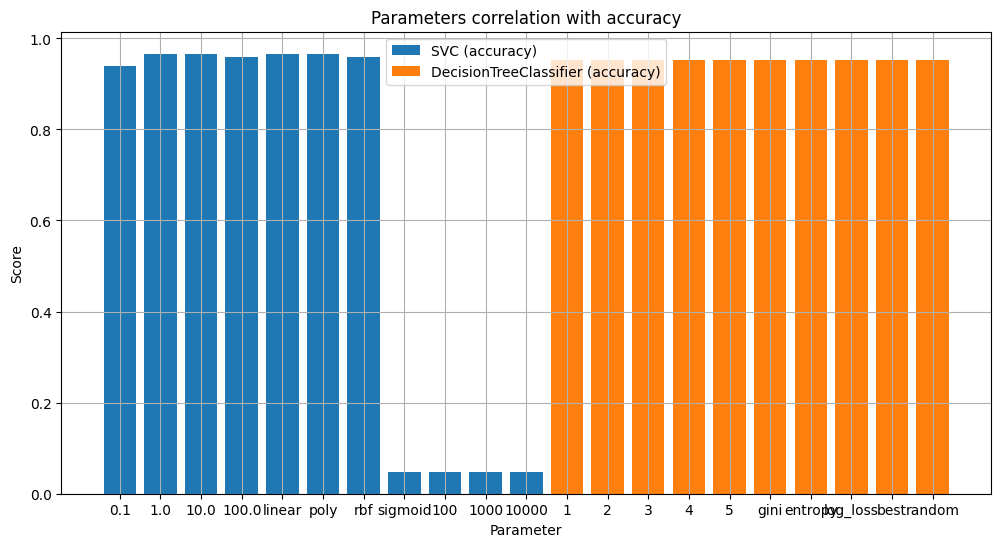
\includegraphics[width=18cm, height=10cm]{output1.png}
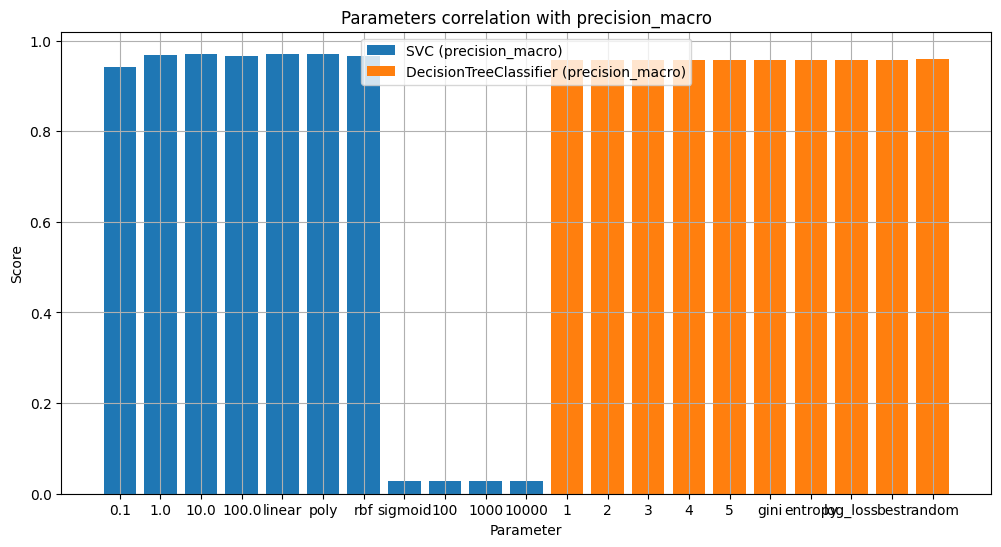
\includegraphics[width=18cm, height=10cm]{output2.png}
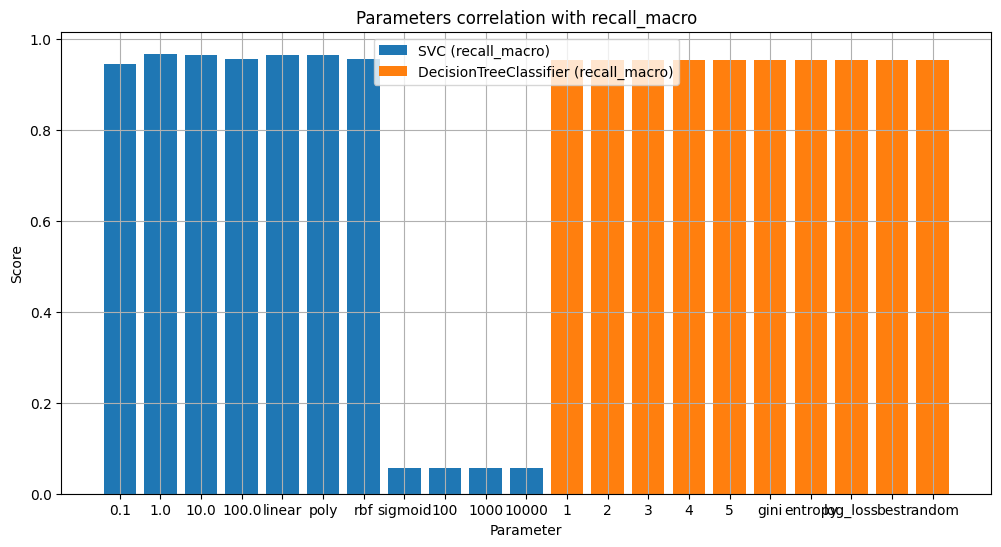
\includegraphics[width=18cm, height=10cm]{output3.png}
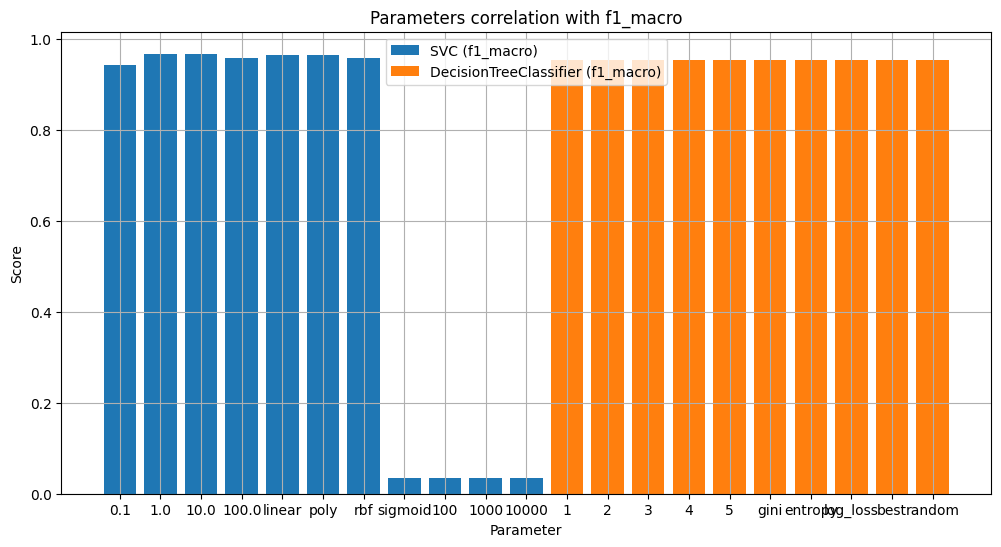
\includegraphics[width=18cm, height=10cm]{output4.png}

\section{Wnioski}

Przy badanych parametrach iteracje nie wpłynęły znacząco na jakość klasyfikacji. Technika podziału jądra sigmoidalnie w SVM okazała się najmniej skuteczna.
Reszta wyników była zbliżona, co sugeruje, że parametry mogły być zbyt mało zróżnicowane, aby wykazać różnice w jakości klasyfikacji.

\end{document}
